\section{Continued use of Scrum}
Group work, especially pair-programming was very important to bring the individual code contributions together. However, the hours of work time spent on the last submission were not distributed as evenly as was the case for the previous submissions as the number of hours increased exponentially during the last 2 weeks before the deadline.
\subsection{Sprints}

\begin{figure}[h]
	\centering
	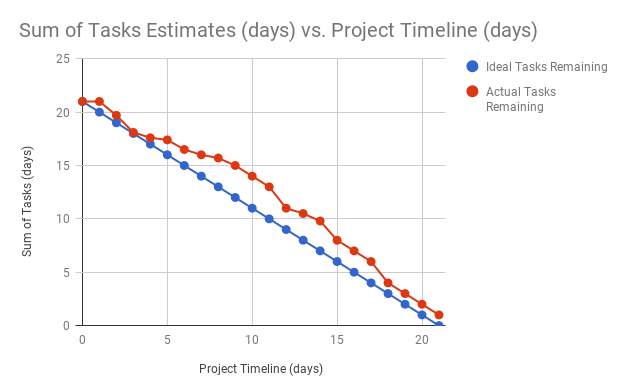
\includegraphics[width=0.6\textwidth]{burndown}
	\caption{A Burndown Chart for the past 14 days.}\label{fig:burn}
\end{figure}
The short time period of 3 weeks meant that we decided to have only 1 sprint and no more role-rotations until the final deadline. During these 3 weeks we met up often to discuss individual task assignments, asses our sprint progress and work on tasks jointly. Although the tasks identified from the initial specifications were not completed to their entirety as discussed earlier, all feasible work was completed in time and progress was made throughout the time period of the sprint.
\subsection{Scrum board}
Unfortunately our previous scrum board was demolished during the srping break, which meant that all user stories had to be redrawn. Appendix \ref{app:board} contains the state of the scrum board at 3 different states - the start of the sprint, the middle and near the deadline. A whiteboard in the John Honey main computer lab was used in order to maintain consistency. 